\section{Creación de UAL Inventarium}
Este es la sección donde se juntan todos los conocimientos y herramientas que hemos ido exponiendo a lo largo de este documentos y los cohesionamos para crear UAL Inventarium.
\\UAL Inventarium o Inventarium es una herramienta web diseñada para la gestión del inventario del Departamento de Informática de la Universidad de Almería.
\\La página web está hecha en Angular 12. Angular es una plataforma de desarrollo compuesta por un framework y librerías. Angular nos brinda todas las herramientas necesarias para la creación de un sitio web.

\subsection{Estructura de un proyecto Angular}
Para poder desplegar un entorno donde trabajar en Angular primero tenemos que instalarlo en nuestro Node Package Manager (NPM) con el siguiente comando:
\begin{verbatim}
    npm i -g @angular/cli
\end{verbatim}
Al hacer esto se nos desplegará nuestro entorno de desarrollo para Angular. El directorio \textbf{node\_modules} es donde se almacena el Framework de Angular, el CLI y los distintos componentes que vayamos instalando con el NPM.
\begin{tcolorbox}
    [colback=green!5!white,colframe=green!75!black,fonttitle=\bfseries,title=¿Qué diferencias hay entre Angular CLI y Angular Framework?]
    Angular CLI es la Command Line Interface la cual permite poder crear proyectos Angular, añadir componentes, servicios o directivas desde una línea de comandos. Angular CLI se encarga de la gestión de las distintas posibilidades que nos puede ofrecer el framework de Angular.
\end{tcolorbox}
Los ficheros que se nos despliegan sobre el directorio raíz al crear un proyecto Angular son:
\begin{itemize}
    \item \textbf{.editorconfig}: Un archivo de configuración para editores de código.
    \item \textbf{README.MD}: Archivo de texto que procesa GitHub en sus repositorios. El contenido inicial del fichero en el momento de la creación del proyecto trata sobre documentación acerca del Framework.
    \item \textbf{angular.json}: Esta es la configuración predeterminada que nos aporta el CLI de Angular para poder construir la aplicación, generar el servicio y testear los diferentes componentes.
    \item \textbf{package.json}: Este fichero se encarga de manejar las dependencias de NPM, precisamente las que están habilitadas dentro del espacio de trabajo.
    \item \textbf{package-lock.json}: Nos aporta información del versionado de los distintos paquetes que están en node\_modules.
    \item \textbf{tsconfig.json}: Esta es la configuración básica de TypeScript para el proyecto.
    \item \textbf{proxy.conf.json}: Este es el fichero que nos va a ayudar a poder consumir nuestra API. Reenvía las peticiones que llegan a nuestra aplicación al puerto 3000 que es donde se encuentra ubicada.
\end{itemize}
En la misma carpeta raíz tenemos un directorio llamado \textit{src}, su descomposición es la siguiente:

\begin{itemize}
    \item \textbf{app}: Directorio que contiene todos los distintos componentes de los que está compuesta la aplicación.
    \item \textbf{assets}: Contiene imágenes y otros recursos para ser copiados en el momento que se construya la aplicación.
    \item \textbf{environments}: Gracias a este fichero podemos configurar una opción en particular de construcción de la aplicación.
    \item \textbf{favicon.ico}: El ícono que sale en la parte superior de la pestaña de la página web.
    \item \textbf{index.html}: La página principal que tiene cualquier web. El CLI se dedica a añadir automáticamente todo el JavaScript y el CSS cuando construye la aplicación. No es un fichero que se use.
    \item \textbf{main.ts}: Este fichero es el punto de entrada principal de la aplicación. Compila la aplicación y arranca el módulo raíz de la aplicación (AppModule) para que se ejecute en el navegador.
    \item \textbf{polyfills.ts}: Provee de adaptaciones para distintos navegadores.
    \item \textbf{styles.css}: Es un archivo de configuración global de estilos para todos los componentes de la aplicación.
    \item \textbf{test.ts}: El punto de entrada principal para los test que se realicen en la aplicación.
\end{itemize}

El contenido del directorio \textit{app} en el momento de la creación del proyecto es el siguiente:

\begin{itemize}
    \item \textbf{app.component.ts}: Define la lógica para la aplicación raíz.
    \item \textbf{app.component.html}: Define el diseño HTML asociaciado con el elemento raíz.
    \item \textbf{app.component.css}: Define el elemento de diseño para el elemento raíz.
    \item \textbf{app.component.spec.ts}: Define el conjunto de pruebas asociado con el elemento raíz.
    \item \textbf{app.module.ts}: Define el módulo raíz, este fichero le comunica a Angular cómo se tiene que realizar el ensamblaje de la aplicación. Inicialmente está declarado detrno de él el propio módulo raíz, pero a medida que vayamos añadiendo elementos a nuestra aplicación irá incluyendo más módulos.
\end{itemize}

Dentro de la carpeta \textit{src} hay tres directorios más:
\begin{itemize}
    \item \textit{components}
    \item \textit{interfaces}
    \item \textit{services}
\end{itemize}

\subsubsection{Componente}
Los componentes son las estructuras principales de construcción que tenemos en Angular. Para poder generarlos utilizamos el siguiente comando:
\begin{verbatim}
    ng g c direccion_y_nombre_del_componente
\end{verbatim}
Cuando lo ejecutemos generará un nuevo directorio con el nombre del componente. Dentro de él se habrán creado cuatro ficheros diferentes:
\begin{itemize}
    \item \textbf{componente.html}: Aquí irá ubicado el diseño html que tendrá el componente.
    \item \textbf{componente.css}: Este documento de estilos se aplicará unicamente al componente.
    \item \textbf{componente.ts}: En nuestro fichero TypeScript tenemos la lógica del componente y cualquier tipo de procesado de datos que haya que realizar.
    \item \textbf{componente.spects.ts}: Este será nuestro fichero de pruebas unitarias para el componente. Durante el desarrollo del proyecto no lo he utilizado ya que el testing del proyecto lo he hecho de otra forma.
\end{itemize}

\subsubsection{Servicio}
Los servicios sirven para aislar más el modelo de vista controlador que presentan los componentes. Estos serán los encargados de comunicarse con nuestra API.
\\Para generar un servicio utilizamos el siguiente comando:
\begin{verbatim}
    ng g s directorio_y_nombre_del_servicio
\end{verbatim}
Se generarán dos ficheros TypeScript, uno para el conjunto de pruebas y otro para el servicio.

\subsubsection{Interfaz}
La interfaz sirve para definir los elementos con los que vamos a trabajar. Estos elementos corresponden a los que tenemos en nuestra base de datos.
\\Para poder generar una interfaz escribimos lo siguiente en la terminal dentro de nuestro proyecto:
\begin{verbatim}
    ng g i directorio_y_nombre_de_la_interfaz
\end{verbatim}
Un ejemplo de interfaz sería por ejemplo la de un objeto del tipo \textit{Configuración}:
\begin{verbatim}
    export interface Configuracion {
        idConfiguracion: number,
        ip: string,
        mac: string,
        boca: string,
        armario: string,
        usuario: string,
        contrasena: string,
        Objeto_idObjeto?: number
    }
\end{verbatim}
Estos elementos también nos ayudarán a procesar las respuestas que nos llegarán desde la API y poder manipularlos en nuestros componentes sin problemas.
\vspace{\baselineskip}
\\Ya sabemos qué tipos de componentes conforman un proyecto Angular. Ahora metemos de lleno las manos en la masa.

\subsection{Disposición y elementos que hay en Inventarium}
Empezaremos hablando de los servicios y las interfaces y cómo se presenta su contenido en el caso de los primeros.

\subsubsection{Interfaces}
Tenemos una interfaz por cada elemento que se encuentra en la base de datos.

\subsubsection{Services}
Los servicios pueden ser los que hayan dado más tipos de problemas a lo largo del desarrollo. Son los encargados de generar las consultas HTTP de las que hemos hablado en la sección anterior en el desarrollo de la API.
\\Tenemos tantos servicios como tablas en la base de datos quitando el de \textit{user} que sirve para iniciar sesión dentro de la aplicación.

\begin{figure}[h]
    \centering
    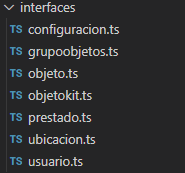
\includegraphics[keepaspectratio]{../contruccion_aplicacion/estructura_del_proyecto/interfaces.png}
    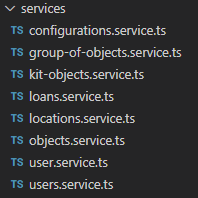
\includegraphics[keepaspectratio]{../contruccion_aplicacion/estructura_del_proyecto/servicios.png}
    \caption{Interfaces y servicios de UAL Inventarium}
\end{figure}



